\documentclass[12pt]{article}

\usepackage{sbc-template}
\usepackage{graphicx,url}
\usepackage{booktabs}
\usepackage[utf8]{inputenc}
\usepackage[T1]{fontenc}
\usepackage[brazil]{babel}
\usepackage[scaled=0.95]{inconsolata}

\sloppy

\title{Análise de Desempenho de ORMs em Consultas SELECT no
  PostgreSQL: uma comparação isolando a camada de abstração entre SQL
  puro, Drizzle e Prisma}

\author{Eduardo Rossetti dos Santos Melo\inst{1}}

\address{Programa de Pós-Graduação em Ciência da Computação\\
  Universidade Estadual Paulista ``Júlio de Mesquita Filho'' (UNESP)
  \email{eduardo.rossetti@unesp.br}
}

\begin{document}

\maketitle

\begin{abstract}
  Object-Relational Mapping (ORM) offers development convenience at the
  cost of an abstraction layer whose performance impact is rarely
  isolated. This work analyzes the performance of two ORM approaches ---
  Drizzle (query builder) and Prisma --- against raw SQL on SELECT
  queries over PostgreSQL, all sharing the same driver (\texttt{pg}) so
  as to isolate the abstraction layer. It combines isolated latency,
  latency under concurrent load (k6, 1/10/100 users), and execution-plan
  analysis across ten scenarios of three query classes. Overhead depends
  on both the query class and the tool's idiom: the query builder is
  negligible on analytical queries ($\approx$1.2$\times$), whereas the
  ORM that materializes the object graph amplifies up to 14$\times$ under
  100 users, by aggregating in the application rather than in the
  database.
\end{abstract}

\begin{resumo}
  O Mapeamento Objeto-Relacional (ORM) oferece conveniência ao custo de
  uma camada de abstração cujo impacto no desempenho é raramente
  isolado. Este trabalho analisa o desempenho de duas abordagens de ORM
  --- Drizzle (query builder) e Prisma --- frente ao SQL puro em
  consultas SELECT no PostgreSQL, todas sobre o mesmo driver
  (\texttt{pg}), isolando a camada de abstração. Combinam-se latência
  isolada, latência sob carga concorrente (k6, 1/10/100 usuários) e
  análise de planos de execução, em dez cenários de três classes. A
  sobrecarga depende da classe da consulta e do idioma da ferramenta: o
  query builder é desprezível em analíticas ($\approx$1,2$\times$),
  enquanto o ORM que materializa o grafo de objetos amplifica até
  14$\times$ sob 100 usuários, por agregar na aplicação em vez de no
  banco.
\end{resumo}

\section{Introdução}

O Mapeamento Objeto-Relacional (\textit{Object-Relational Mapping} ---
ORM) é um padrão consolidado para acesso a bancos de dados relacionais
em sistemas orientados a objetos, permitindo que desenvolvedores
manipulem dados por meio de construções da própria linguagem de
programação, sem redigir manualmente as instruções em SQL
(\textit{Structured Query Language}) \cite{nicoletti2024}. Sua principal
vantagem é elevar o nível de abstração do acesso a dados: o foco do
desenvolvimento desloca-se para o modelo de domínio, reduzindo o código
repetitivo e facilitando a manutenção \cite{oliveira2024}. Não por
acaso, ferramentas de ORM tornaram-se onipresentes no ecossistema de
desenvolvimento \textit{backend}, em particular no ambiente Node.js,
onde bibliotecas como Prisma, Sequelize e Drizzle figuram entre os
pacotes mais utilizados.

Essa conveniência, contudo, não é gratuita. A camada de mediação decorre
da impedância objeto-relacional (\textit{object-relational impedance
mismatch}) --- o atrito entre o modelo orientado a objetos e o relacional
---, e é na tradução automática de chamadas de método para SQL que reside
a sobrecarga de desempenho, pois o desenvolvedor passa a exercer pouco
controle sobre a eficiência das consultas geradas \cite{nicoletti2024}. A
literatura documenta anti-padrões recorrentes, como o problema N+1, em
que uma operação é decomposta em uma sucessão de consultas linha a linha,
e a busca ansiosa (\textit{eager fetching}) de dados desnecessários
\cite{colley2020}.

Diversos estudos avaliaram empiricamente o desempenho de ORMs, e há
consenso recorrente de que o acesso via SQL puro supera o acesso mediado
por ORM em operações básicas \cite{yusmita2025,colley2020}. Entretanto,
três limitações enfraquecem a comparabilidade desses trabalhos. Primeiro,
comparações que confrontam múltiplos ORMs frequentemente misturam a
sobrecarga (overhead) da abstração com a do \textit{driver} de banco,
pois cada ferramenta utiliza um driver distinto --- um fator de confusão
(\textit{confounder}) que contamina a atribuição de causa. Segundo, boa
parte dos estudos concentra-se em operações CRUD simples ou em médias
agregadas, sem decompor o comportamento por classe de consulta nem
investigar como a sobrecarga evolui sob carga concorrente. Terceiro, são
raras as análises que recorrem ao plano de execução (\textit{EXPLAIN
ANALYZE}) como evidência causal do porquê de uma estratégia ser mais
lenta que outra, limitando-se a reportar tempos sem explicá-los.

Este trabalho aborda essas lacunas comparando, de forma controlada, três
abordagens de acesso a dados em consultas SELECT sobre o PostgreSQL: SQL
puro (via \textit{driver} \texttt{pg}), Drizzle (um \textit{query
builder}, que constrói SQL de forma programática sem mapear entidades) e
Prisma (um ORM completo). A decisão metodológica central é submeter todas
as abordagens
ao \textbf{mesmo driver de banco} (\texttt{pg}), de maneira a isolar
exclusivamente a camada de abstração e neutralizar o confound do driver
presente em estudos anteriores. A avaliação articula-se em três camadas
complementares de medição --- latência isolada, latência sob carga
concorrente com 1, 10 e 100 usuários virtuais, e análise de planos de
execução ---, aplicadas a dez cenários que cobrem três classes de
consulta (simples, anti-padrão e analítica), em ambiente containerizado
com geração sintética e determinística de dados, à maneira de
\cite{yusmita2025}.

A pesquisa é norteada pela pergunta: \textit{qual é a sobrecarga de
utilizar um ORM em vez de SQL puro em consultas SELECT no PostgreSQL, e
como ela varia conforme a classe da consulta e a carga concorrente?} A
hipótese é que a sobrecarga não é uniforme, mas depende tanto da classe
quanto do idioma da ferramenta --- modesta para um \textit{query builder}
que emite SQL equivalente, mas amplificada sob carga para um ORM que
materializa o grafo de objetos em memória. Os resultados confirmam a
hipótese e, por meio dos planos de execução, identificam o mecanismo
causal da degradação.

O artigo segue com a fundamentação teórica (Seção 2), os trabalhos
relacionados (Seção 3), a arquitetura experimental (Seção 4), os
resultados e as ameaças à validade (Seção 5) e as conclusões (Seção 6).

\section{Fundamentação}

\subsection{Do driver ao ORM: um espectro de abstração}

O acesso a um banco relacional situa-se em diferentes níveis de
abstração. No nível mais baixo, o \textit{driver} executa SQL escrito
manualmente, oferecendo controle total ao custo de código repetitivo e
acoplado ao banco. Em nível intermediário, os \textit{query builders}
constroem SQL de forma programática e tipada, sem mapear entidades,
emitindo tipicamente uma consulta por operação. No nível mais alto, os
ORMs completos mapeiam tabelas a objetos de domínio e expõem uma API
declarativa \cite{nicoletti2024}. O ORM eleva o nível de abstração e
reduz a duplicação \cite{oliveira2024}; sua contrapartida é que, ao gerar
consultas automaticamente, deixa o desenvolvedor com pouco controle sobre
a eficiência do SQL produzido \cite{nicoletti2024}.

\subsection{Impedância objeto-relacional}

A impedância objeto-relacional é o atrito entre dois modelos
estruturalmente distintos: o orientado a objetos --- uma rede de objetos
com identidade e estado, percorrida por navegação --- e o relacional ---
declarativo e baseado em conjuntos, no qual cada operação resulta em uma
nova relação \cite{teixeira2017}. \cite{ireland2009} distinguem quatro
níveis de impedância (paradigma, linguagem, esquema e instância) e
estimam que de 25\% a 50\% do código de uma aplicação objeto-relacional
se dedique a transpô-los. O ORM é o conjunto de estratégias que
automatizam essa ponte.

\subsection{Anti-padrões em consultas geradas por ORM}

Por gerar SQL automaticamente, os ORMs tendem a reproduzir anti-padrões
reconhecidos na literatura \cite{colley2020}. O mais citado é o problema
N+1, em que uma operação resolvível por uma única consulta baseada em
conjuntos é decomposta em uma sucessão de consultas linha a linha;
somam-se a ele a busca ansiosa (\textit{eager fetching}) de dados
desnecessários e a preferência por subconsultas aninhadas em vez de
junções. Como consultas baseadas em conjuntos são mais eficientes que
acessos linha a linha \cite{colley2020}, é a violação desse princípio que
caracteriza boa parte da sobrecarga atribuída aos ORMs.

\subsection{O plano de execução como instrumento de análise}

No PostgreSQL, o SQL é declarativo: o otimizador baseado em custo decide
\textit{como} executar a consulta, produzindo um plano de execução. O
comando \texttt{EXPLAIN ANALYZE} reporta a estrutura do plano e os tempos
reais de planejamento e execução. Comparar o plano e o número de
consultas emitidas por um ORM com os de uma consulta manual permite
explicar \textit{por que} uma é mais lenta que a outra --- instrumento
pouco explorado nos estudos comparativos de desempenho de ORMs.

\subsection{As ferramentas avaliadas: Prisma e Drizzle}

No ecossistema Node.js, o Prisma figura entre os ORMs mais adotados para
TypeScript e JavaScript \cite{oliveira2024}. Diferentemente dos ORMs
clássicos baseados nos padrões \textit{Active Record} ou \textit{Data
Mapper}, o Prisma define o modelo de dados em um arquivo de esquema
próprio (\texttt{schema.prisma}), a partir do qual gera um cliente
fortemente tipado, acessado por uma API declarativa de alto nível, que
carrega relações aninhadas por junções laterais (\textit{preview feature}
\texttt{relationJoins}) \cite{prisma2025}. O Drizzle, por sua vez, é uma
biblioteca mais recente e deliberadamente mais leve, classificada como
\textit{query builder}: oferece uma API tipada próxima da sintaxe do
próprio SQL, sem mapear entidades de domínio nem manter um
\textit{runtime} de mediação, emitindo tipicamente uma única consulta
por operação \cite{drizzle2025}. Essa diferença de propósito --- um ORM
completo, que materializa o grafo de objetos, \textit{versus} um
\textit{query builder}, que apenas constrói o SQL --- é central para a
interpretação dos resultados das Seções 5.2 e 5.3.

\section{Trabalhos Relacionados}

A comparação de desempenho entre ORMs e SQL puro é objeto de diversos
estudos empíricos, com consenso de que o acesso direto supera o mediado
por ORM. A referência mais próxima é \cite{yusmita2025}, que compara SQL
puro e o ORM Prisma sobre o PostgreSQL, com dados sintéticos, e conclui
que o SQL puro é até cinco vezes mais rápido e consome de seis a nove
vezes menos CPU. \cite{colley2020} confrontam consultas escritas por
especialista com as geradas pelo Django ORM, relatando um caso em que o
ORM emite mais de mil consultas onde o SQL emprega uma única. No contexto
brasileiro e em Node.js, \cite{oliveira2024} comparam TypeORM, Prisma e
Sequelize em operações CRUD sob carga (k6), sobre um esquema de comércio
eletrônico semelhante ao adotado aqui; e \cite{couto2022} avaliam o
PostgreSQL sob carga concorrente, com uma análise de ameaças à validade
que serve de referência. O rigor metodológico apoia-se ainda em trabalhos
sobre \textit{benchmarking} confiável
\cite{kalibera2013,beyer2017,hasselbring2021}.

Três lacunas frente a esses estudos justificam a contribuição. Primeiro,
estudos que
comparam múltiplos ORMs frequentemente os apoiam em \textit{drivers}
distintos, confundindo a sobrecarga da abstração com a do driver
\cite{oliveira2024}; ao unificar o driver, isolamos exclusivamente a
camada de abstração. Segundo, a maioria reporta médias agregadas ou
restringe-se a operações CRUD, sem decompor o comportamento por classe
de consulta nem observar sua evolução sob diferentes níveis de carga.
Terceiro, são raras as análises que empregam o plano de execução como
evidência causal das diferenças observadas.

\section{Arquitetura Experimental}

Esta seção descreve a arquitetura experimental adotada para avaliar o
desempenho das abordagens de acesso a dados. O delineamento privilegia a
reprodutibilidade e o isolamento de variáveis: o ambiente é integralmente
containerizado, os dados são gerados de forma determinística e cada
abordagem é medida em isolamento de processo, conforme detalhado a
seguir.

\subsection{Ambiente de testes}

Os experimentos rodaram em uma única máquina, para eliminar a
variabilidade de rede entre cliente e servidor: processador AMD Ryzen 7
7700X (8 núcleos, 16 \textit{threads}), 32 GB de RAM e SSD NVMe, sob
Ubuntu 26.04 LTS. O PostgreSQL 17.9 \cite{postgresql} executou em
contêiner Docker (extensão \texttt{pg\_stat\_statements} habilitada,
demais parâmetros padrão); a aplicação rodou sobre o Node.js 24, e a
carga concorrente foi gerada pelo k6 \cite{k6}. As versões das
bibliotecas foram fixadas para reprodutibilidade: \texttt{pg} 8.20,
Drizzle 0.45.2 e Prisma 7.8. O uso de contêineres é prática recomendada
para benchmarks confiáveis \cite{beyer2017,yusmita2025}.

\subsection{Esquema relacional e geração de dados}

O esquema reproduz um domínio de comércio eletrônico com cinco tabelas
relacionadas --- \texttt{users}, \texttt{addresses}, \texttt{products},
\texttt{carts} e \texttt{cart\_items} (Figura 1) ---, com chaves
estrangeiras (e exclusão em cascata) e índices secundários sobre as
colunas mais consultadas. É definido por um \textit{script} SQL único,
que constitui a fonte da verdade; o modelo do Prisma e o esquema do
Drizzle apenas o espelham, garantindo que as três abordagens operem sobre
estruturas idênticas.

\begin{figure}[!htb]
\centering
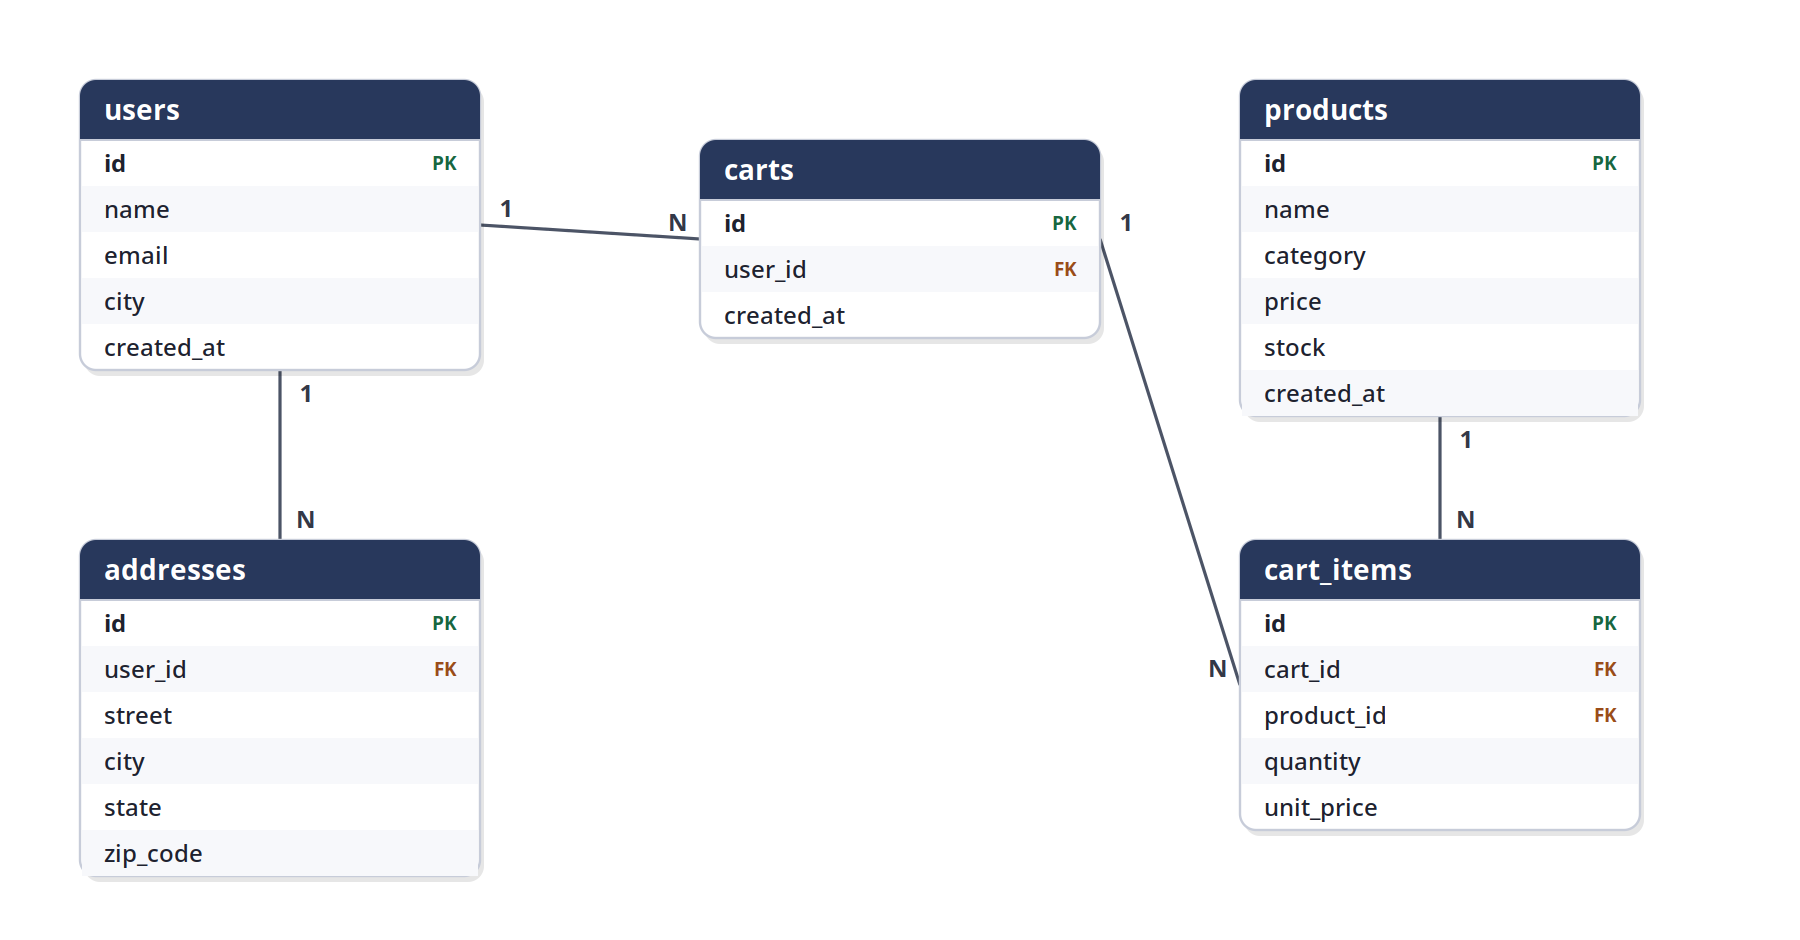
\includegraphics[width=.72\textwidth]{figures/modelo-er.png}
\caption{Modelo entidade-relacionamento do esquema}
\label{fig:er}

\vspace{2pt}{\footnotesize Fonte: elaboração própria.}
\end{figure}

Os dados foram gerados com a biblioteca \textit{faker.js} sob semente
fixa (\texttt{faker.seed(12345)}), tornando o conjunto determinístico e
reproduzível \cite{yusmita2025}. Para evitar uniformidade artificial,
adotou-se uma distribuição assimétrica de carrinhos por usuário (cerca de
30\% sem carrinho e uma cauda de compradores frequentes), com datas
distribuídas nos 90 dias anteriores à geração. O volume final é de 10.000
usuários, 10.000 endereços, 1.100 produtos (100 nunca vendidos), 13.195
carrinhos e 46.018 itens de carrinho --- cerca de 80 mil registros ---,
escolhido para que o tempo do banco não dominasse a medição, tornando
visível a sobrecarga da abstração.

Entre cada medição, o estado do banco é restaurado a partir de um
\textit{snapshot} em formato CSV (via \texttt{TRUNCATE \ldots{} RESTART
IDENTITY CASCADE} seguido de \texttt{COPY}, \texttt{ANALYZE} e
\texttt{CHECKPOINT}), prática padrão em \textit{benchmarks} de banco de
dados para garantir que cada execução parta de um estado idêntico e
controlado. Todo o material --- código, dados sintéticos, scripts e
resultados consolidados --- está disponível publicamente no repositório
do projeto, com versões fixadas e geração determinística
(\texttt{faker.seed(12345)}), garantindo a reprodutibilidade.

\subsection{Abordagens avaliadas}

Foram avaliadas três abordagens de acesso a dados, todas operando sobre o
\textbf{mesmo driver} \texttt{pg} (node-postgres). Essa uniformização é a
decisão metodológica central do trabalho: ao manter o driver constante,
isola-se exclusivamente o custo da camada de abstração, neutralizando o
fator de confusão presente em estudos que comparam ORMs apoiados em
drivers distintos. A Tabela 1 resume as abordagens, cujos conceitos foram
apresentados na Seção 2.5.

\begin{table}[!htb]
\centering
\caption{Abordagens de acesso a dados avaliadas}
\label{tab:abordagens}
\scriptsize
\begin{tabular}{@{}p{2.0cm}p{2.0cm}p{1.7cm}p{6.0cm}@{}}
\toprule
Abordagem & Tipo & Biblioteca & Caminho de acesso \\
\midrule
\texttt{sql} & Driver direto (SQL puro) & pg 8.20 & \texttt{pool.query} com SQL e parâmetros (\texttt{\$1, \$2, \ldots}) \\
\texttt{drizzle} & \textit{Query builder} & Drizzle 0.45.2 & API programática que emite uma única consulta SQL \\
\texttt{prisma} & ORM completo (idiomático) & Prisma 7.8 & API declarativa; com \texttt{relationJoins}, carrega relações por \textit{LATERAL JOIN} \\
\bottomrule
\end{tabular}

\vspace{2pt}{\footnotesize Fonte: elaboração própria.}
\end{table}

A abordagem \texttt{sql} é o limite inferior de sobrecarga (acesso direto
ao driver) e o Drizzle emite uma única consulta SQL por operação. O Prisma
foi avaliado em seu uso idiomático (\texttt{prisma}), sem recurso a SQL
bruto: para consultas que sua API declarativa não expressa nativamente,
recorre-se ao caminho natural da ferramenta --- recuperar os registros e
processá-los na aplicação ---; e, com a \textit{preview feature}
\texttt{relationJoins}, carrega relações aninhadas por \textit{LATERAL
JOIN} em uma única consulta.

\subsection{Cenários e classes de consulta}

A avaliação cobre dez cenários de consulta SELECT, agrupados em três
classes que representam perfis distintos de acesso a dados (Tabela 2). As
consultas de \textbf{escrita foram deliberadamente excluídas} do escopo,
pois nelas o custo do ORM mistura-se à divergência da primitiva
expressável (por exemplo, atualização em massa em uma consulta versus
$N$ atualizações em transação), o que confunde a atribuição da
sobrecarga à camada de abstração; além disso, operações de escrita produzem planos
de execução triviais, pouco informativos para a análise causal
pretendida. Cada cenário foi implementado de forma idiomática em todas as
abordagens, e sua equivalência semântica foi verificada automaticamente
antes da coleta (comparando contagem de linhas, identificadores e
agregados, tomando o SQL puro como referência).

\begin{table}[!htb]
\centering
\caption{Cenários por classe de consulta}
\label{tab:cenarios}
\scriptsize
\begin{tabular}{@{}p{1.6cm}p{4.3cm}p{6.4cm}@{}}
\toprule
Classe & Cenário & Padrão de consulta \\
\midrule
Simples & \texttt{select\_by\_id} & busca por chave primária \\
Simples & \texttt{cart\_detail} & JOIN de um nível com filtro de linha única \\
Anti-padrão & \texttt{n\_plus\_one} & 100 consultas seriais (uma por carrinho) \\
Anti-padrão & \texttt{eager\_join} & mesmo resultado em uma única consulta (\texttt{IN} + LEFT JOIN) \\
Analítica & \texttt{revenue\_by\_city\_and\_category} & JOIN de 5 tabelas + GROUP BY + \texttt{SUM(a$\cdot$b)} + COUNT DISTINCT + AVG \\
Analítica & \texttt{recent\_carts\_7d} & varredura por faixa em índice B-tree de \textit{timestamp} + JOIN \\
Analítica & \texttt{frequently\_bought\_together} & auto-junção (\textit{SELF-JOIN}) + GROUP BY + COUNT \\
Analítica & \texttt{products\_never\_sold} & \texttt{NOT EXISTS} correlacionado \\
Analítica & \texttt{browse\_catalog\_paginated} & CTE \textit{top-N} + JOIN + paginação por \texttt{OFFSET} \\
Analítica & \texttt{users\_above\_avg\_spending} & \texttt{HAVING} com subconsulta escalar \\
\bottomrule
\end{tabular}

\vspace{2pt}{\footnotesize Fonte: elaboração própria.}
\end{table}

As consultas simples representam o caso de menor custo no banco, no qual
a sobrecarga da camada de abstração tende a ser proporcionalmente mais
visível. Os anti-padrões contrastam, propositadamente, uma implementação
deficiente (\texttt{n\_plus\_one}, com 100 consultas seriais) com sua
forma equivalente em consulta única (\texttt{eager\_join}), permitindo
observar como cada abordagem se comporta diante de um padrão
reconhecidamente custoso. As consultas analíticas exercitam recursos do
SQL --- junções de múltiplas tabelas, agregações compostas, subconsultas
escalares e funções de janela ---, nos quais o tempo de processamento do
banco é maior e, em princípio, dominante.

\subsection{Métricas e protocolo de medição}

A avaliação articula-se em três camadas complementares de medição, de
modo a capturar o desempenho sob óticas distintas.

\textbf{Camada 1 --- Latência isolada.} Mede-se o tempo de execução de
cada cenário em um processo Node dedicado, sem servidor HTTP, executando
200 iterações medidas precedidas de 50 iterações de aquecimento
(\textit{warmup}) descartadas, com o banco restaurado entre cenários.
Reporta-se a mediana e o 95º percentil, em consonância com a recomendação
de privilegiar a mediana em medições de desempenho sujeitas a ruído
\cite{kalibera2013}. Essa camada estabelece a latência de referência,
livre de efeitos de concorrência.

\textbf{Camada 2 --- Latência sob carga.} Cada abordagem é exposta por um
servidor HTTP (Fastify) e submetida a carga concorrente gerada pelo k6,
em três níveis de usuários virtuais simultâneos (1, 10 e 100 VUs), por 30
segundos cada. Para permitir a estimativa de dispersão entre execuções,
cada combinação (abordagem $\times$ cenário $\times$ nível de VU) foi
repetida em \textbf{três réplicas}, totalizando uma matriz de 3 $\times$
10 $\times$ 3 $\times$ 3 = 270 execuções; reporta-se a mediana entre
réplicas. Registram-se a latência (p50, p95), a vazão
(\textit{throughput}, em requisições por segundo) e a taxa de erro, com um limiar de aceitação de menos de 1\% de
falhas.

\textbf{Camada 3 --- Análise de planos.} Para investigar a \textit{causa}
das diferenças de desempenho, captura-se o SQL efetivamente emitido por
cada abordagem (por interceptação do driver) e executa-se \texttt{EXPLAIN
(ANALYZE, BUFFERS)} sobre cada consulta, reportando o tempo de
planejamento e de execução no banco, bem como o \textbf{número de
consultas} disparadas por operação. Essa última métrica é decisiva para
evidenciar anti-padrões como a decomposição de uma operação em múltiplas
consultas \cite{colley2020}.

A métrica primária de comparação é a \textbf{razão de sobrecarga}
(\textit{overhead ratio}) entre cada ORM e o SQL puro (ORM/SQL); valores
acima de 1$\times$ indicam que o ORM é mais lento. Para sumarizar por
classe de consulta, utiliza-se a média geométrica das razões, mais
apropriada do que a média aritmética para agregar fatores
multiplicativos.

\subsection{Isolamento de processo}

Em testes preliminares, carregar múltiplas abordagens em um mesmo
processo Node introduzia viés sob carga: a abordagem baseada no driver
puro sofria degradação muito maior que as demais, por contenção no laço
de eventos (\textit{event loop}) de thread única quando vários
\textit{pools} de conexão operam em paralelo. Para mitigar isso,
\textbf{cada abordagem executa em um processo Node dedicado}, e o servidor
é reiniciado a cada combinação (abordagem $\times$ cenário $\times$ VU),
evitando contaminação cruzada por um \textit{pool} degradado. Esse
isolamento das execuções individuais é apontado como indispensável para
benchmarks confiáveis \cite{beyer2017} e constitui, em si, um diferencial
metodológico frente a estudos que não controlam essa fonte de viés.

\section{Resultados e Discussão}

A matriz completa compreendeu 270 execuções de carga, além da latência
isolada e da análise de planos para as trinta combinações de abordagem e
cenário. Das 270 células, 269 transcorreram sem qualquer falha; a única
exceção é discutida na Seção 5.5 e constitui um artefato estatístico, não
uma falha de medição. Os resultados são organizados das três camadas de
medição para a evidência causal: latência isolada (5.1), comportamento
sob carga (5.2) e planos de execução (5.3).

\subsection{Latência isolada}

A Tabela 3 reúne a latência isolada (\texttt{bench.js}): a mediana do SQL
puro, em milissegundos, e a sobrecarga de cada ORM expressa como razão em
relação a ela ($\times$SQL).

\begin{table}[!htb]
\centering
\caption{Latência isolada (\texttt{bench.js}): mediana do SQL puro e sobrecarga dos ORMs ($\times$SQL) por cenário}
\label{tab:bench}
\scriptsize
\begin{tabular}{@{}llrrr@{}}
\toprule
Classe & Cenário & SQL p50 (ms) & Drizzle & Prisma \\
\midrule
Simples & \texttt{select\_by\_id} & 0,107 & 1,67$\times$ & 2,04$\times$ \\
Simples & \texttt{cart\_detail} & 0,157 & 1,56$\times$ & 1,63$\times$ \\
Anti-padrão & \texttt{n\_plus\_one} & 9,248 & 1,14$\times$ & 1,49$\times$ \\
Anti-padrão & \texttt{eager\_join} & 0,593 & 2,47$\times$ & 6,06$\times$ \\
Analítica & \texttt{revenue\_by\_city\_and\_category} & 75,78 & 1,02$\times$ & 3,86$\times$ \\
Analítica & \texttt{recent\_carts\_7d} & 0,904 & 1,21$\times$ & 3,90$\times$ \\
Analítica & \texttt{frequently\_bought\_together} & 0,360 & 1,27$\times$ & 2,38$\times$ \\
Analítica & \texttt{products\_never\_sold} & 0,723 & 1,11$\times$ & 1,18$\times$ \\
Analítica & \texttt{browse\_catalog\_paginated} & 4,011 & 1,00$\times$ & 1,03$\times$ \\
Analítica & \texttt{users\_above\_avg\_spending} & 27,32 & 1,09$\times$ & 3,22$\times$ \\
\bottomrule
\end{tabular}

\vspace{2pt}{\footnotesize Fonte: elaboração própria.}
\end{table}

O Drizzle mantém-se muito próximo do SQL puro em todas as classes: a
sobrecarga é modesta nas simples (1,56--1,67$\times$) e praticamente
desaparece nas analíticas, chegando a empatar com o SQL onde o tempo do
banco domina (1,00$\times$ em \texttt{browse\_catalog\_paginated})
--- coerente com um \textit{query builder} que emite SQL equivalente ao
manual. O Prisma, ao contrário, já revela sobrecarga apreciável mesmo sem
concorrência: contida nas simples (1,63--2,04$\times$), mas acentuada no
anti-padrão \texttt{eager\_join} (6,06$\times$) e nas analíticas com
agregação (3,86$\times$ em \texttt{revenue\_by\_city\_and\_category};
3,22$\times$ em \texttt{users\_above\_avg\_spending}); já em analíticas
sem agregação na aplicação, como \texttt{products\_never\_sold}
(1,18$\times$), permanece próximo do SQL --- contraste que antecipa o
mecanismo causal da Seção 5.3.

\subsection{Latência sob carga}

Sob carga concorrente, o padrão observado isoladamente amplifica-se, e de
modo desigual entre as ferramentas. A Figura 2 traça a trajetória da
sobrecarga média (média geométrica das razões ORM/SQL) por classe de
consulta ao longo dos três níveis de carga, e a Figura 3 apresenta a
vazão por cenário sob 100 usuários virtuais.

\begin{figure}[!htb]
\centering
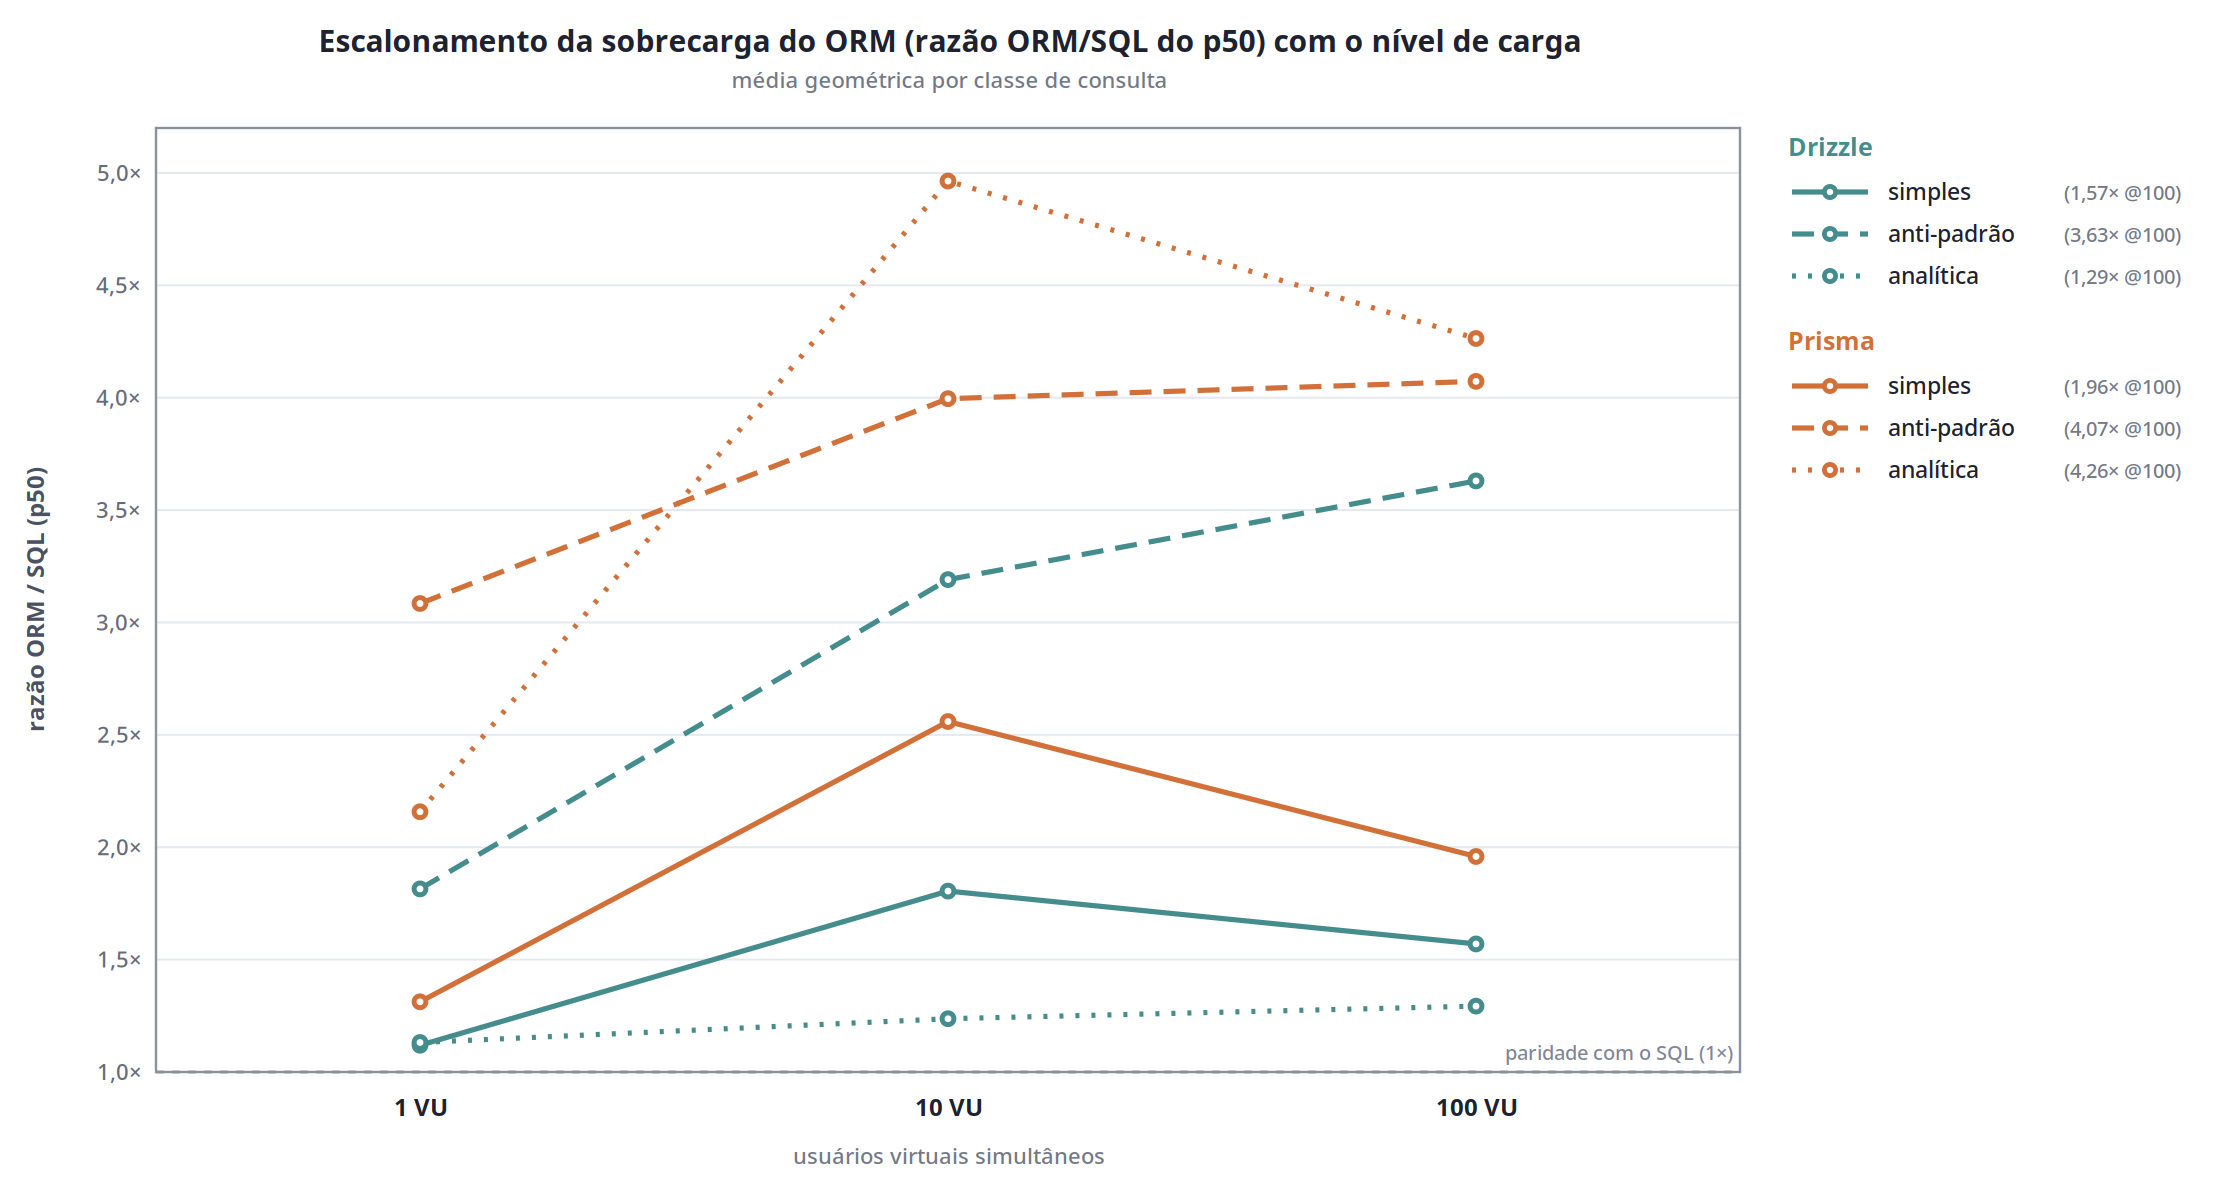
\includegraphics[width=.82\textwidth]{figures/escalonamento-overhead.png}
\caption{Escalonamento da sobrecarga (média geométrica da razão ORM/SQL do p50) por classe de consulta e nível de carga}
\label{fig:escalonamento}

\vspace{2pt}{\footnotesize Fonte: elaboração própria.}
\end{figure}

A Figura 2 torna visível o achado central: as duas analíticas seguem
trajetórias opostas. A do Drizzle (linha pontilhada) permanece rente à
paridade com o SQL em qualquer carga (de 1,13$\times$ a 1,29$\times$), ao
passo que a do Prisma escala de 2,16$\times$ (1 VU) para 4,96$\times$ (10
VUs). As consultas simples de ambas as ferramentas formam um arco ---
sobem de 1 para 10 VUs e recuam a 100 VUs, quando o tempo do banco passa
a dominar ---, enquanto o anti-padrão cresce de forma monotônica com a
carga nas duas ferramentas.

\begin{figure}[!htb]
\centering
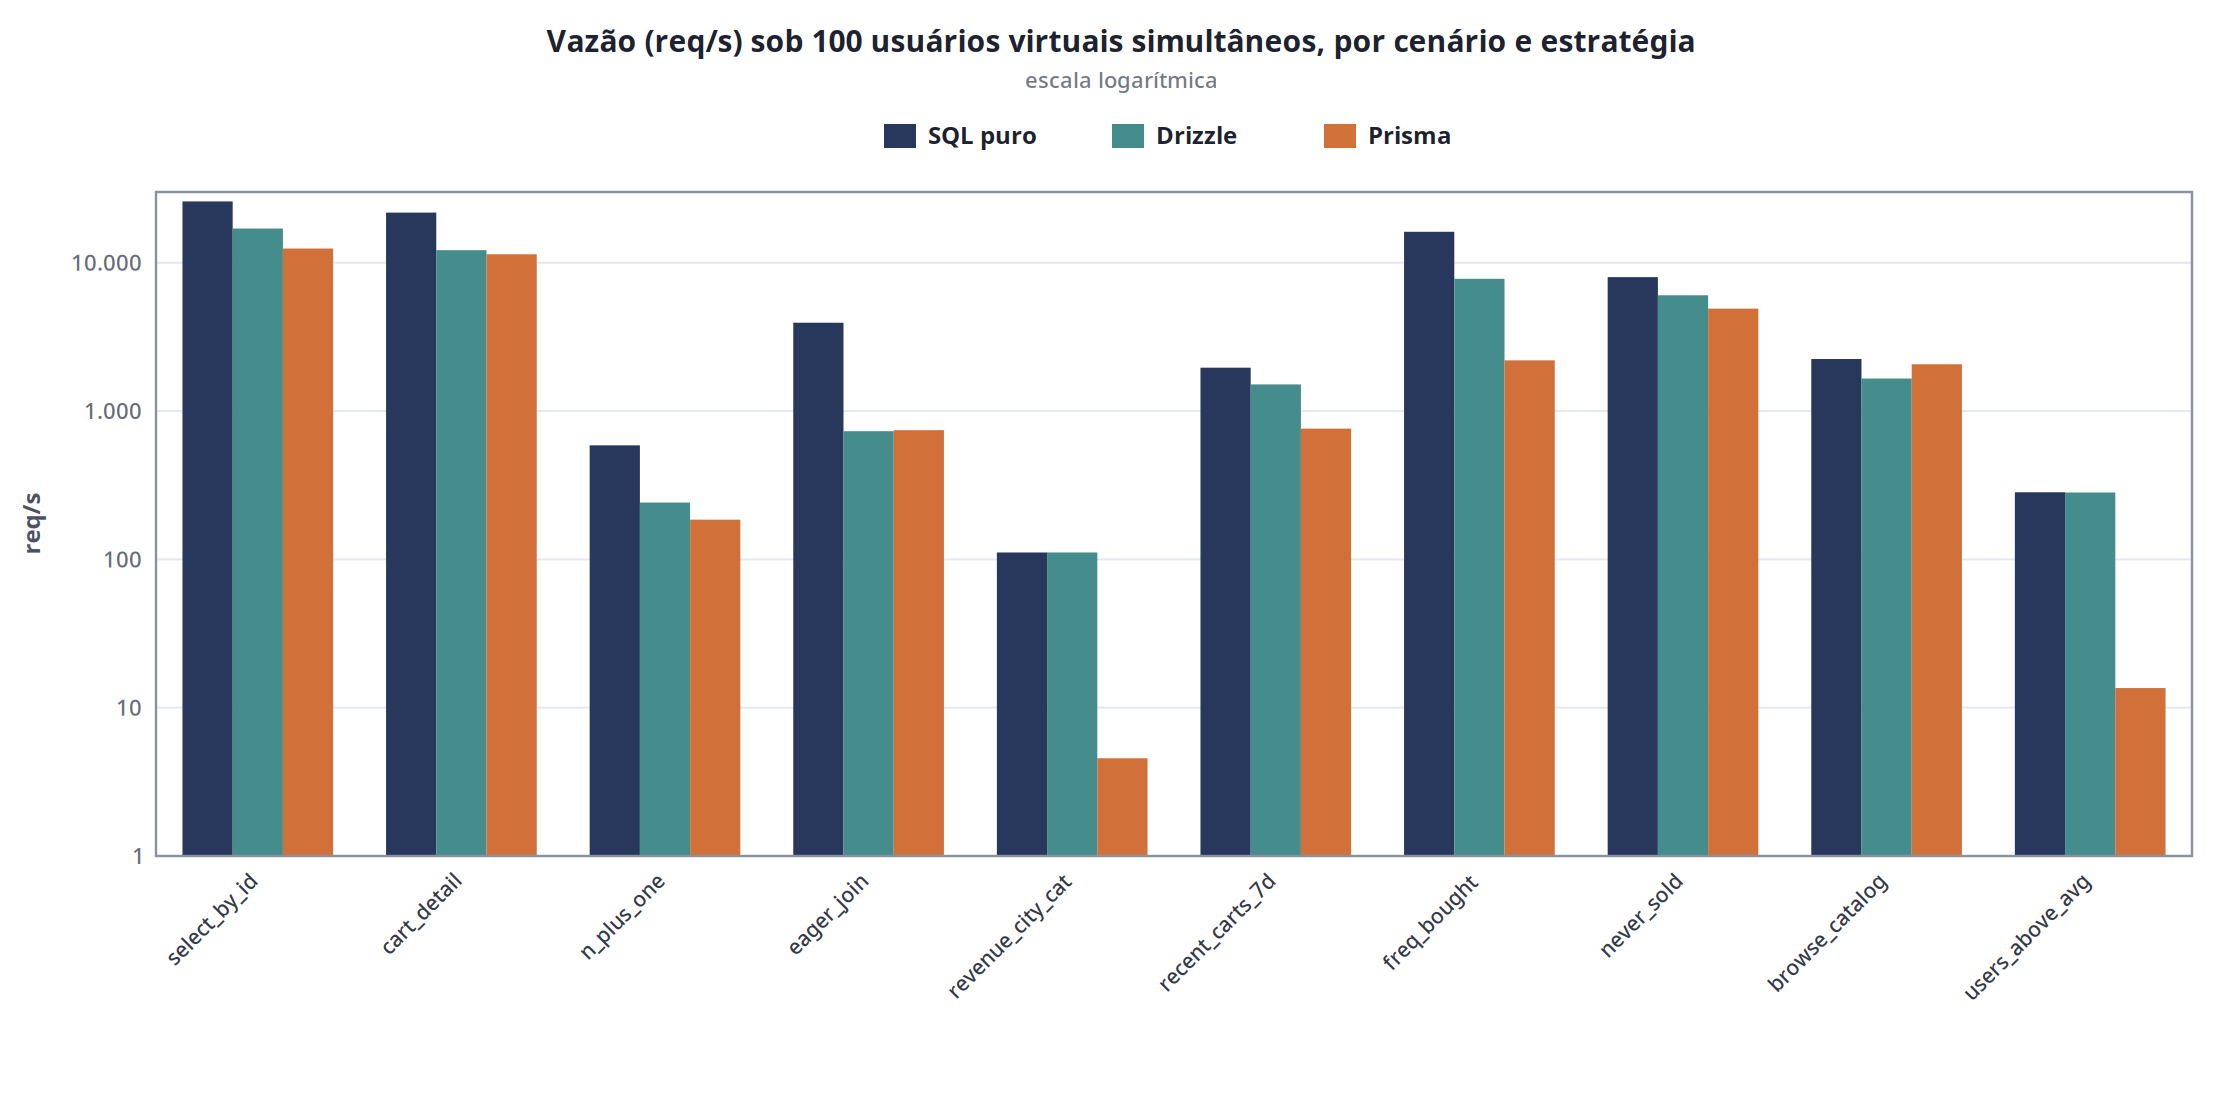
\includegraphics[width=.85\textwidth]{figures/vazao-100vu.png}
\caption{Vazão (req/s) sob 100 usuários virtuais simultâneos, por cenário e abordagem}
\label{fig:vazao}

\vspace{2pt}{\footnotesize Fonte: elaboração própria.}
\end{figure}

Três observações sobressaem. Primeiro, o Drizzle preserva sobrecarga
desprezível nas analíticas mesmo sob carga máxima (1,29$\times$ a 100
VUs): quando o ORM emite o mesmo SQL, o custo da abstração dilui-se à
medida que o tempo do banco domina. Segundo, o Prisma exibe o oposto ---
a sobrecarga analítica salta de 2,16$\times$ (1 VU) para 4,96$\times$ (10
VUs), e sob 100 VUs a razão Prisma/SQL chega a \textbf{12,73$\times$ em
\texttt{revenue\_by\_city\_and\_category}} (5 contra 111 req/s) e
\textbf{14,43$\times$ em \texttt{users\_above\_avg\_spending}} (14 contra
284 req/s), como nas barras truncadas da Figura 3. Terceiro, no
anti-padrão ambas amplificam sob carga (3,63$\times$ e 4,07$\times$ a 100
VUs): o ORM \textbf{não corrige} o N+1 --- ao contrário, agrava-o, por
pagar o custo da abstração a cada consulta serial. Em síntese, a
sobrecarga do ORM depende \textbf{tanto da classe da consulta quanto do
idioma da ferramenta}: um \textit{query builder} que delega a computação
ao banco é desprezível nas analíticas, enquanto um ORM que materializa o
grafo de objetos na aplicação inverte essa propriedade e degrada sob
carga.

\subsection{Evidência causal: planos de execução}

A contagem de consultas emitidas explica os números acima. O SQL puro e o
Drizzle emitem exatamente \textbf{uma} consulta por operação em todos os
cenários (exceto o \texttt{n\_plus\_one}, deficiente por construção em
qualquer abordagem), com planos estruturalmente idênticos --- o que
explica por que o Drizzle acompanha o SQL puro tão de perto. A degradação analítica do Prisma idiomático, contudo,
\textbf{não} decorre de decomposição em múltiplas consultas: com
\texttt{relationJoins}, ele emite uma única consulta com \textit{LATERAL
JOIN}. A causa é outra: em cenários como
\texttt{revenue\_by\_city\_and\_category} e
\texttt{users\_above\_avg\_spending}, a API declarativa do Prisma não
expressa a agregação composta (somas de produtos, médias de somas,
contagens distintas), de modo que o caminho idiomático recupera
\textbf{todos} os registros pertinentes (dezenas de milhares de linhas) e
realiza a agregação em JavaScript, em vez de delegá-la ao banco. Sob
concorrência, esse processamento na aplicação --- somado à serialização
do grande volume de dados --- satura o laço de eventos, produzindo a
latência de mais de 11 segundos observada a 100 VUs. É um mecanismo
distinto, porém complementar, do clássico anti-padrão de decomposição em
$N$ consultas relatado na literatura, em que um ORM chega a emitir mais
de mil consultas onde o SQL emprega uma \cite{colley2020}.

O Quadro 1 detalha esse mecanismo em
\texttt{users\_above\_avg\_spending}. O SQL puro e o Drizzle resolvem tudo
em uma única consulta cuja agregação (\texttt{SUM}, \texttt{AVG},
\texttt{HAVING}) e recorte (\texttt{LIMIT 50}) ocorrem no banco,
devolvendo \textbf{apenas 50 linhas} (38,1 ms). O Prisma idiomático, sem
API para essa agregação, emite uma consulta que materializa \textbf{as
46.018 linhas} de itens e refaz a agregação em JavaScript: a varredura
custa modestos 27 ms no banco, mas é a transferência e o processamento
desse volume na aplicação que, sob concorrência, produzem a latência de
p50 de cerca de 5 s a 100 VUs.

\vspace{6pt}
\noindent\textbf{Quadro 1 --- SQL emitido em
\texttt{users\_above\_avg\_spending}: agregação no banco (SQL/Drizzle)
vs.\ materialização em JavaScript (Prisma)}
\vspace{2pt}

{\scriptsize
\begin{verbatim}
-- (a) SQL puro e Drizzle - 1 consulta; agregacao resolvida no banco:
SELECT u.id, u.name, SUM(ci.quantity * ci.unit_price) AS spent
FROM users u
  JOIN carts      c  ON c.user_id = u.id
  JOIN cart_items ci ON ci.cart_id = c.id
GROUP BY u.id, u.name
HAVING SUM(ci.quantity * ci.unit_price) > (
         SELECT AVG(s.spent) FROM (
           SELECT SUM(ci.quantity * ci.unit_price) AS spent
           FROM cart_items ci JOIN carts c ON c.id = ci.cart_id
           GROUP BY c.user_id) s)
ORDER BY spent DESC LIMIT 50;
-- Plano: HashAggregate + top-N heapsort -> 50 linhas retornadas

-- (b) Prisma idiomatico - consulta que materializa TODOS os itens
--     (sem SUM/GROUP BY/HAVING); agregacao refeita em JavaScript.
--     A relacao 'cart' vem por LEFT JOIN LATERAL sobre carts:
SELECT t0.id, t0.quantity, t0.unit_price, cart
FROM cart_items AS t0
  LEFT JOIN LATERAL (
    SELECT jsonb_build_object('userId', t1.user_id)
    FROM carts AS t1 WHERE t0.cart_id = t1.id LIMIT 1) AS cart ON true;
-- Plano: Nested Loop Left Join -> 46.018 linhas retornadas
-- (+ 2a consulta trivial buscando os nomes dos 50 usuarios escolhidos)
\end{verbatim}
}

\noindent{\footnotesize Fonte: elaboração própria, a partir dos planos
capturados em \texttt{results/explain/}.}

\vspace{6pt}

\subsection{Ameaças à validade}

Algumas ameaças à validade devem ser ponderadas. Cliente (k6) e servidor
compartilham a mesma máquina, o que pode introduzir contenção sob 100
VUs; optou-se por isso para eliminar a variabilidade de rede e, como a
métrica primária é a razão entre abordagens --- todas sujeitas à mesma
contenção ---, o viés afeta numerador e denominador de forma comparável.
Sob o k6, a ordem de chegada das requisições concorrentes é
não-determinística, mas a métrica reportada é a mediana sobre milhares de
requisições, o que dilui assimetrias de sequência. A única célula que
acusou violação do limiar de erro
(\texttt{prisma}/\texttt{revenue\_by\_city\_and\_category}/100 VUs) teve
taxa de falha real nula --- é consequência da própria lentidão do Prisma
(mais de 11 s de latência), um achado, não um defeito. Por fim, avaliou-se
uma versão de cada ferramenta; como o Drizzle é uma das abstrações mais
leves, sua sobrecarga pode ser lida como um \textbf{limite inferior} para
a de ORMs em geral, e a concordância entre as medições isoladas e sob 1 VU
reforça a validade interna do isolamento de processo.

\section{Conclusões}

Mediar o acesso a dados por um ORM tem um preço em desempenho que, na
literatura, costuma ser reportado como um número único e sem explicação
causal. Este trabalho analisou esse desempenho de forma controlada ---
comparando SQL puro, Drizzle e Prisma em consultas SELECT no PostgreSQL
--- e, mais do que quantificar a sobrecarga, buscou identificar de que
ela depende: a classe da consulta e a carga concorrente. A principal
decisão metodológica --- submeter todas as abordagens ao mesmo
\textit{driver} (\texttt{pg}) --- permitiu isolar a camada de abstração e
atribuir a ela, e não ao driver, as diferenças observadas; e a
combinação de três camadas de medição com a análise de planos de execução
possibilitou não apenas quantificar, mas explicar a sobrecarga.

Os resultados confirmam e refinam a hipótese inicial: \textbf{a
sobrecarga do ORM depende tanto da classe da consulta quanto do idioma da
ferramenta}. O Drizzle, um \textit{query builder} que emite SQL
equivalente ao manual, apresenta sobrecarga modesta e, sobretudo,
desprezível nas consultas analíticas mesmo sob carga máxima (1,29$\times$
em média a 100 VUs), pois delega a computação ao banco. O Prisma, em sua
forma idiomática, inverte essa propriedade: por materializar o grafo de
objetos e realizar agregações na própria aplicação, amplifica
drasticamente sob carga, alcançando 12 a 14 vezes a latência do SQL puro
em consultas analíticas a 100 usuários simultâneos. A análise dos planos
de execução revelou a origem dessa degradação: o processamento de
agregações em memória, na própria aplicação, em vez de no banco.
Observou-se ainda que o ORM \textbf{não corrige} anti-padrões como o N+1,
mas os agrava.

Desses achados decorre uma recomendação prática: o ORM custa mais caro
justamente onde tende a ser mais necessário --- em consultas analíticas
sob alta concorrência ---, de modo que aplicações sensíveis a desempenho
nesse perfil beneficiam-se de um \textit{query builder} ou de SQL puro
para suas consultas críticas, evitando delegar à aplicação agregações que
o banco realiza de forma muito mais eficiente.

\bibliographystyle{sbc}
\bibliography{referencias}

\end{document}
